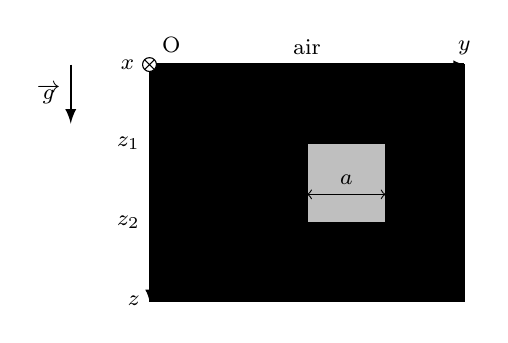
\begin{tikzpicture} [
	scale=1,
	font=\footnotesize,
	force/.style={->,>=latex,draw=\JRLblue,very thick,nodes={\JRLblue}},
	vecteur/.style={-latex,thick},
	liquide/.style={fill=\JRLblueC,very thin,draw=\JRLblueF},
    solide/.style={fill=lightgray}
	]
	% liquide
%	\shadedraw[color=gray,top color=white,bottom color=gray] (-2,0)--++(4,0)--++(0,-3)--++(-4,0)--cycle;
	\draw[liquide] (-2,0)--++(4,0)--++(0,-3)--++(-4,0)--cycle;
	\draw[line width=1pt] (-2,0)--++(4,0);
	\draw (0,0) node[below]{liquide ($\rho$)};
	\draw (0,0) node[above]{air};
	% solide
	\draw[solide,shift={(0,-2)}](0,0)rectangle(1,1);
	\draw[shift={(0,-2)},<->](0,10pt)--++(1,0)node[midway,above]{$a$};
	% forces
	\draw[vecteur] (-3,0)--++(0,-0.75) node[pos=0.5,left]{$\overrightarrow{g}$};
	\draw[shift={(0,-2)},force](-.5,.5)--++(.5,0);
	\draw[shift={(0,-2)},force](1.5,.5)--++(-.5,0);
	\draw[shift={(0,-2)},force](.5,1.4)--++(0,-.4);
	\draw[shift={(0,-2)},force](.5,-.7)--++(0,.7);	
	% axes
	\draw[->,>=latex,shift={(-2,0)}](0,0)node[above right=1pt]{O}--++(0,-3)node[left]{$z$};
	\draw[->,>=latex,shift={(-2,0)}](0,0)--++(4,0)node[above]{$y$};
	\draw[fill=white,shift={(-2,0)}](0,0)circle(2.5pt)node[left=2pt]{$x$};
	\draw[shift={(-2,0)}](0,0)(45:2.5pt)--(225:2.5pt)(-45:2.5pt)--(135:2.5pt);
	\draw[dashed,shift={(-2,-1)}](0,0)node[left]{$z_1$}--(2,0);
	\draw[dashed,shift={(-2,-2)}](0,0)node[left]{$z_2$}--(2,0);
\end{tikzpicture}